\hsection{Getting the Examples from this Book}%
%
\begin{figure}%
\centering%
\tightbox{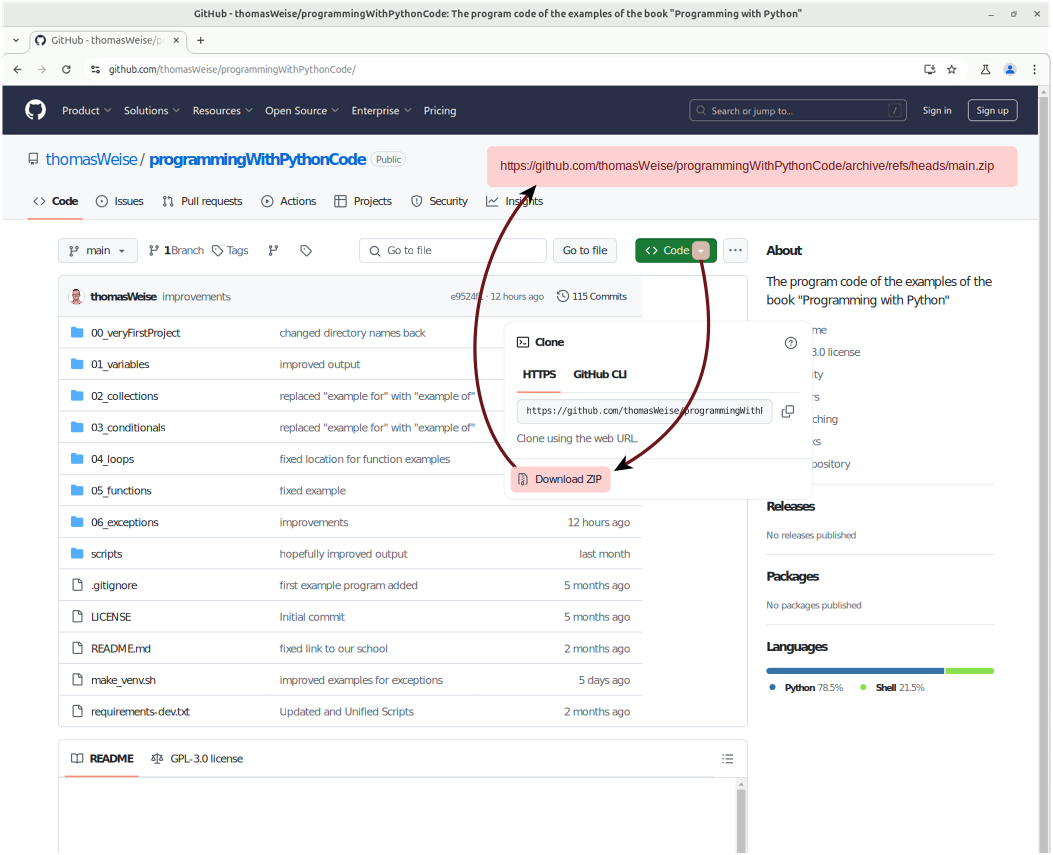
\includegraphics[width=0.8\linewidth,trim={0pt 1cm 0pt 0pt},clip]{\currentDir/downloadExamples}}%
\caption{%
Downloading all the example source codes as a single \texttt{zip}~archive from \expandafter\url{\programmingWithPythonCodeRepo}.}%
\label{fig:downloadExamples}%
\end{figure}%
%
\begin{figure}%
\centering%
%
\subfloat[][%
Click \menu{Clone Repository} in the \pycharm\ welcome screen.%
\label{fig:clone01welcomeToPycharm}%
]{\tightbox{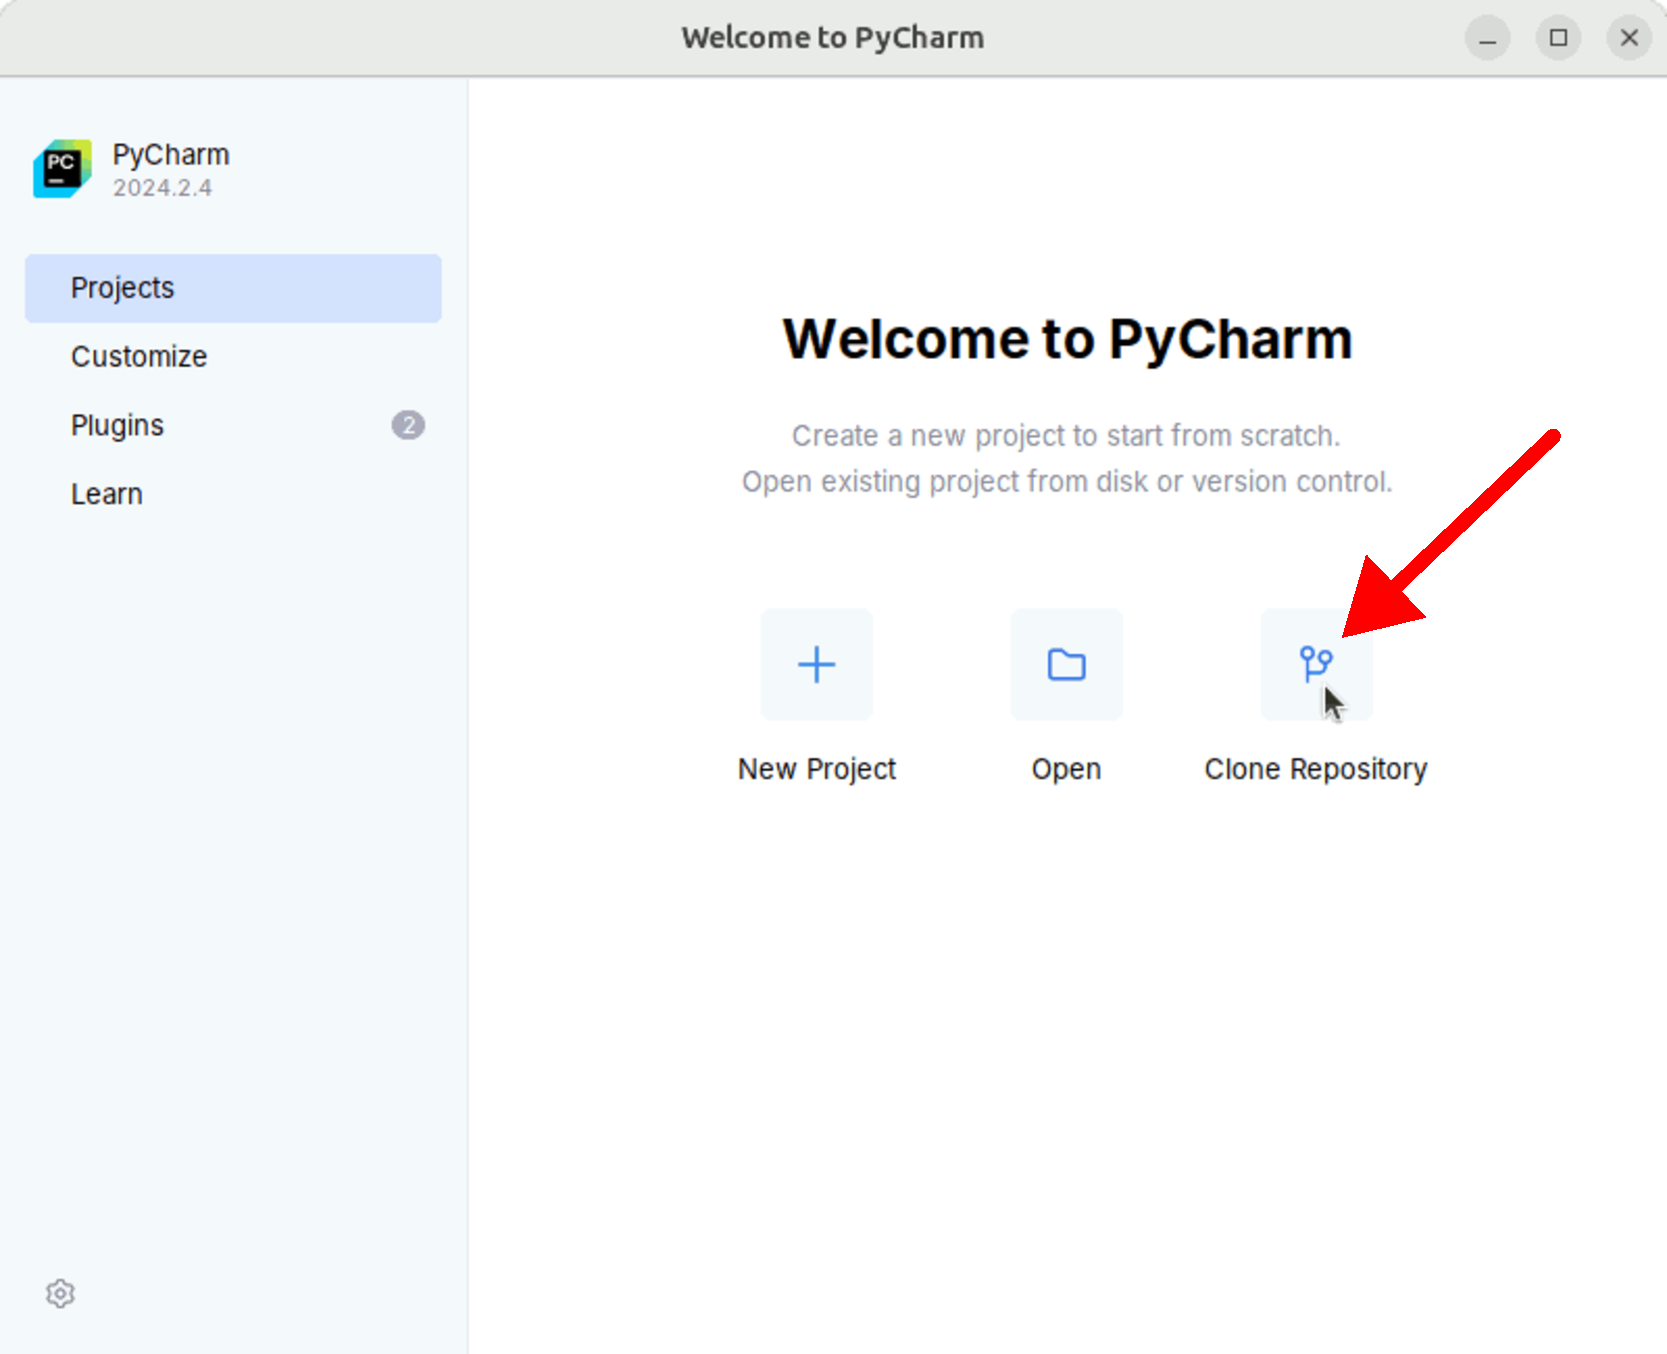
\includegraphics[width=0.45\linewidth]{\currentDir/clone01welcomeToPycharm}}}%
%
\floatSep%
%
\subfloat[][%
Selecting \menu{URL:} \expandafter\url{\programmingWithPythonCodeRepo} and a reasonable destination \menu{Directory:} in the next dialog, then click \menu{Clone}.%
\label{fig:clone02selectRepoAndDestination}%
]{\tightbox{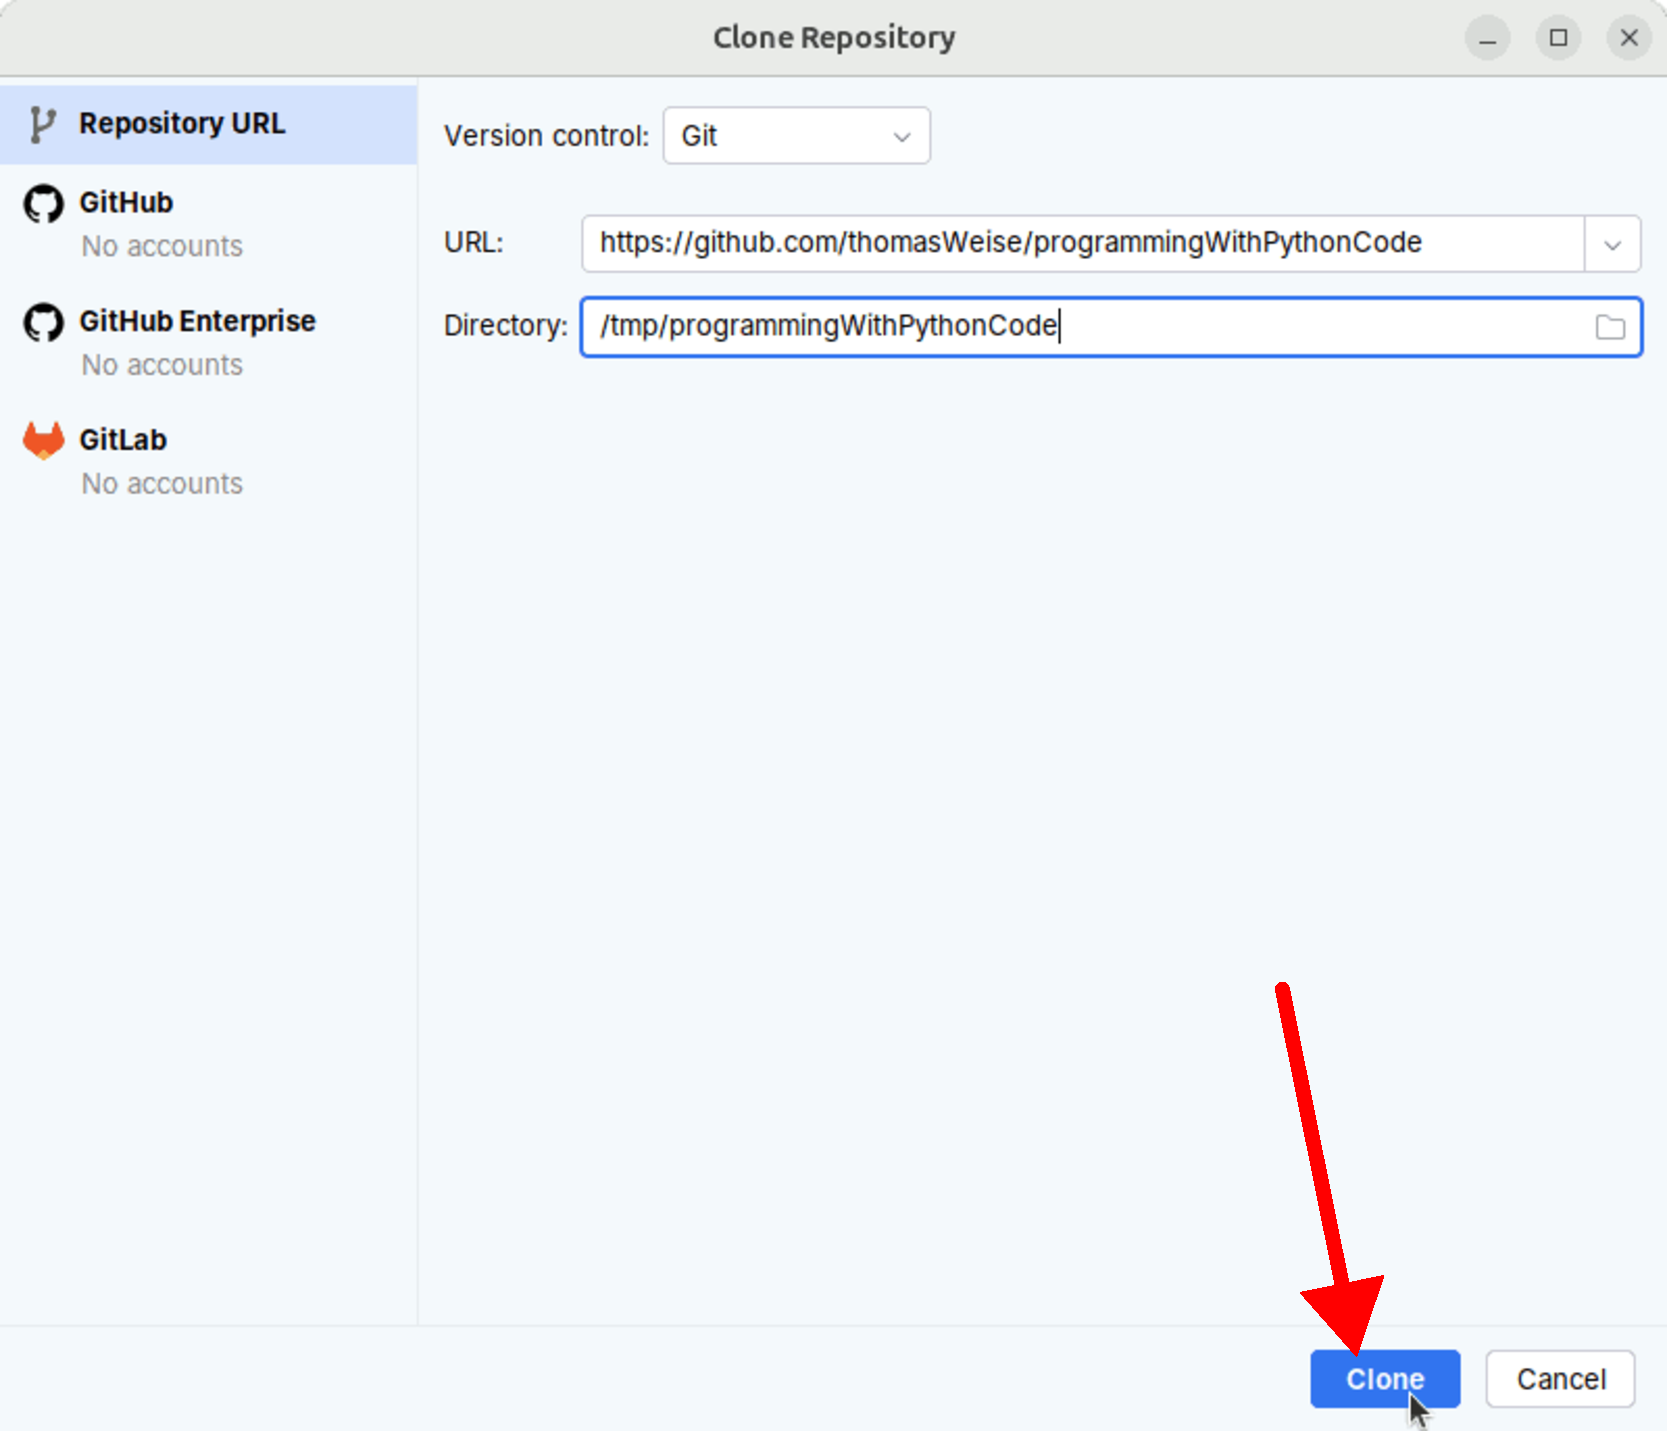
\includegraphics[width=0.45\linewidth]{\currentDir/clone02selectRepoAndDestination}}}%
%
\floatRowSep%
%
\subfloat[][%
Wait while \pycharm\ is cloning (downloading) the repository.%
\label{fig:clone03cloning}%
]{\tightbox{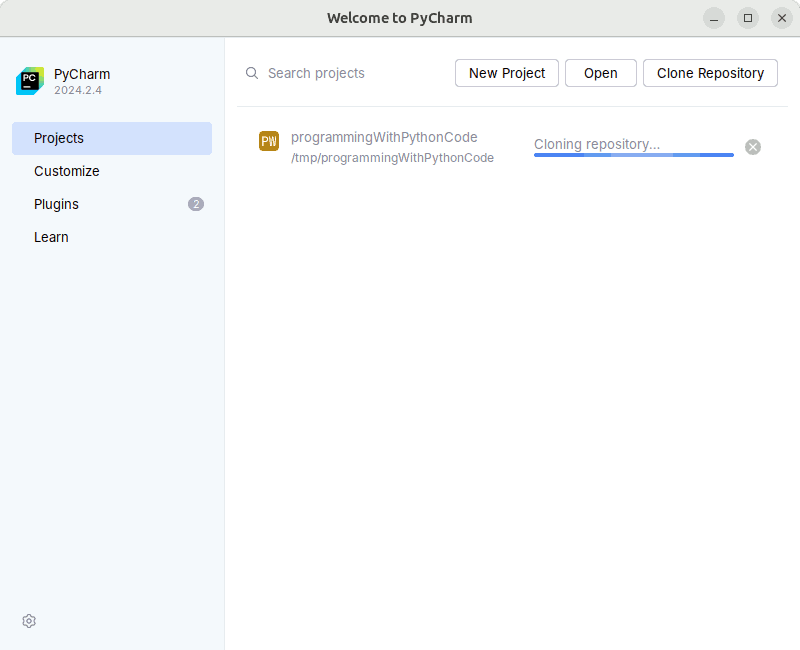
\includegraphics[width=0.45\linewidth]{\currentDir/clone03cloning}}}%
%
\floatSep%
%
\subfloat[][%
If asked, click \menu{Trust Project} after confirming that you indeed downloaded the right code and if you trust our code.%
\label{fig:clone04trustProject}%
]{\tightbox{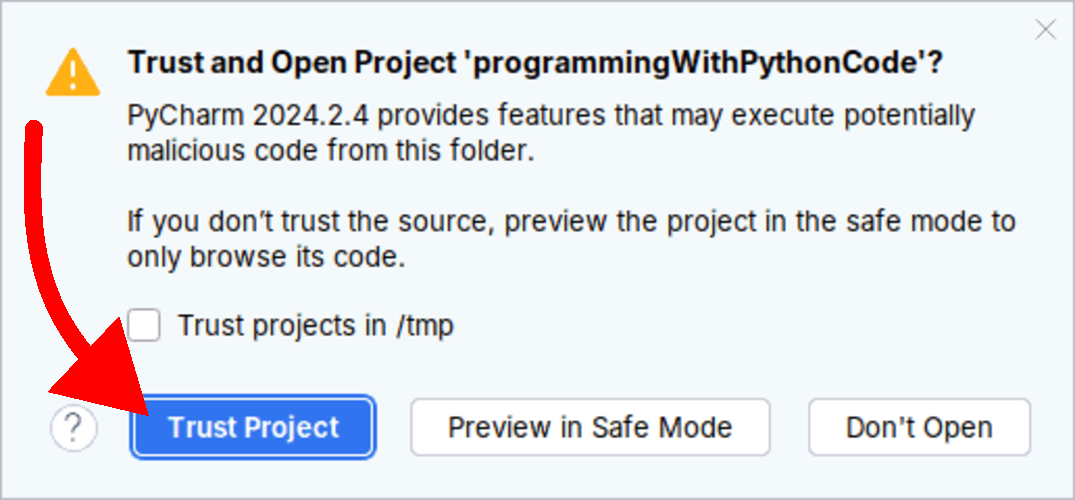
\includegraphics[width=0.45\linewidth]{\currentDir/clone04trustProject}}}%
%
\floatRowSep%
%
\subfloat[][%
The project with all the examples from this book is now downloaded and can be accessed in \pycharm.%
\label{fig:clone05finished}%
]{\tightbox{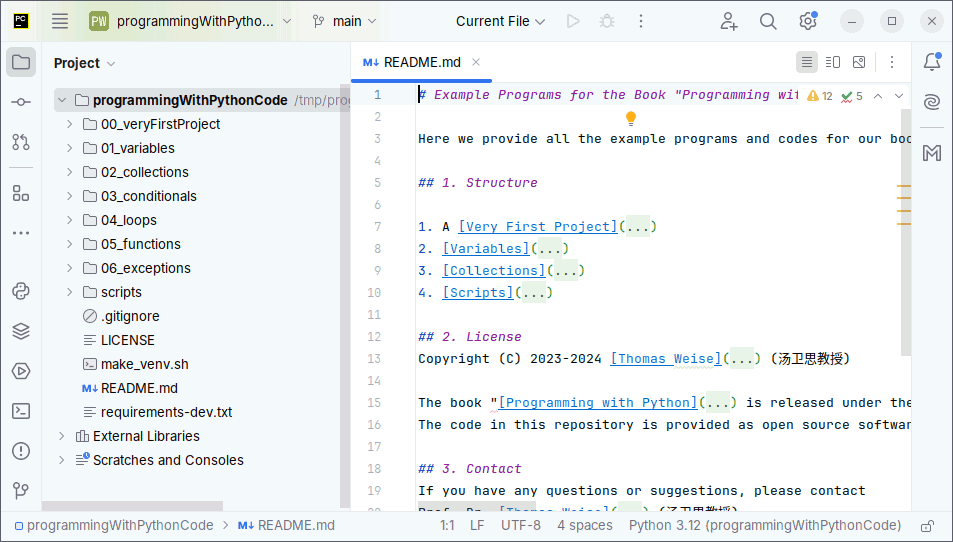
\includegraphics[width=0.6\linewidth]{\currentDir/clone05finished}}}%
%
\caption{Using \pycharm\ to clone (download) and import all the examples from this book.}%
\label{fig:cloningExamples}%
\end{figure}%
%
This book comes with a lot of examples programs written in \python.
While our first explorations of the simple data types will mainly use the \python\ console, we will later almost exclusively write programs in \python\ files.
Every single one of them is available in the \pgls{git} repository \texttt{\programmingWithPythonCodeRepoName}.
You can directly access this repository at \pgls{github} under \expandafter\url{\programmingWithPythonCodeRepo}.%
%
\begin{sloppypar}%
On the website, you can directly download all the examples as illustrated in \cref{fig:downloadExamples}.
First, you would click on the little downward facing triangle in the button \menu{Code}.
This will open a small dialog \menu{Clone} in which you can click on the \menu{Download ZIP} button.
This, in turn, enters the URL~\expandafter\url{\programmingWithPythonCodeRepo/archive/refs/heads/main.zip} into your browser's download queue.
A \texttt{zip}~archive is a single file that can contain other files and folders and can be opened by the standard file managers both on \ubuntu\ and \windows.
Once downloaded, the archive contains all the examples that we use in our book.%
\end{sloppypar}%
%
\begin{sloppypar}%
Alternatively to downloading a \texttt{zip} archive with the examples from this book, you can also directly create a new project in \pycharm\ by cloning (basically, downloading) the repository as illustrated in \cref{fig:cloningExamples}.
In the \pycharm\ welcome screen, you click \menu{Clone Repository} as shown in \cref{fig:clone01welcomeToPycharm}.
In the next dialog, you have to select a source \menu{URL:}, which will be \expandafter\url{\programmingWithPythonCodeRepo}.
You also need to choose a \menu{Directory:} where the new project should be located.
All the contents of the examples repository will be downloaded into this directory as well.
In \cref{fig:clone02selectRepoAndDestination}, I selected \textil{/tmp/programmingWithPythonCode}, i.e., a directory on my partition for temporary files.
This directory will be cleared at every system boot, so you would certainly choose a more reasonable destination.
After clicking \menu{Clone}, the downloading will begin, as sketched in \cref{fig:clone03cloning}.%
\end{sloppypar}%
%
Once the repository has been downloaded, \pycharm\ may ask you whether you trust this project.
After making sure that you indeed downloaded the examples for this book (and if you deem this code trustworthy), you can click \menu{Trust Project}, as \cref{fig:clone04trustProject}.
Finally, as \cref{fig:clone05finished} shows, you can now see and play with and run all the examples in \pycharm.%
%
\endhsection%
%
